\documentclass{ctexart}

\usepackage{amsmath}
\usepackage{amssymb}
\usepackage{amsfonts}
\usepackage{listings}
\usepackage{tikz}
\usetikzlibrary{automata,positioning}

\usepackage{color}

\definecolor{mygreen}{rgb}{0,0.6,0}
\definecolor{mygray}{rgb}{0.5,0.5,0.5}
\definecolor{mymauve}{rgb}{0.58,0,0.82}

\lstset{ %
	backgroundcolor=\color{white},   % choose the background color; you must add \usepackage{color} or \usepackage{xcolor}
	basicstyle=\footnotesize,        % the size of the fonts that are used for the code
	breakatwhitespace=false,         % sets if automatic breaks should only happen at whitespace
	breaklines=true,                 % sets automatic line breaking
	captionpos=b,                    % sets the caption-position to bottom
	commentstyle=\color{mygreen},    % comment style
	deletekeywords={...},            % if you want to delete keywords from the given language
	escapeinside={\%*}{*)},          % if you want to add LaTeX within your code
	extendedchars=true,              % lets you use non-ASCII characters; for 8-bits encodings only, does not work with UTF-8
	frame=single,	                   % adds a frame around the code
	keepspaces=true,                 % keeps spaces in text, useful for keeping indentation of code (possibly needs columns=flexible)
	keywordstyle=\color{blue},       % keyword style
	language=Octave,                 % the language of the code
	otherkeywords={*,...},           % if you want to add more keywords to the set
	numbers=left,                    % where to put the line-numbers; possible values are (none, left, right)
	numbersep=5pt,                   % how far the line-numbers are from the code
	numberstyle=\tiny\color{mygray}, % the style that is used for the line-numbers
	rulecolor=\color{black},         % if not set, the frame-color may be changed on line-breaks within not-black text (e.g. comments (green here))
	showspaces=false,                % show spaces everywhere adding particular underscores; it overrides 'showstringspaces'
	showstringspaces=false,          % underline spaces within strings only
	showtabs=false,                  % show tabs within strings adding particular underscores
	stepnumber=1,                    % the step between two line-numbers. If it's 1, each line will be numbered
	stringstyle=\color{mymauve},     % string literal style
	tabsize=2,	                   % sets default tabsize to 2 spaces
	title=\lstname                   % show the filename of files included with \lstinputlisting; also try caption instead of title
}

\lstdefinestyle{customc}{
	belowcaptionskip=1\baselineskip,
	breaklines=true,
	frame=L,
	xleftmargin=\parindent,
	language=C,
	showstringspaces=false,
	basicstyle=\footnotesize\ttfamily,
	keywordstyle=\bfseries\color{green!40!black},
	commentstyle=\itshape\color{purple!40!black},
	identifierstyle=\color{blue},
	stringstyle=\color{orange},
}

\lstdefinestyle{customasm}{
	belowcaptionskip=1\baselineskip,
	frame=L,
	xleftmargin=\parindent,
	language=[x86masm]Assembler,
	basicstyle=\footnotesize\ttfamily,
	commentstyle=\itshape\color{purple!40!black},
}

\lstset{escapechar=@,style=customc}

\title{Advanced Software Engineering HW6}
\author{吴俊宇 15212880}

\begin{document}

\maketitle

\section*{Problem 1 LTL2GeneralizedBchi}

Produce Buchi Automaton for \lstinline|(false U p)|.

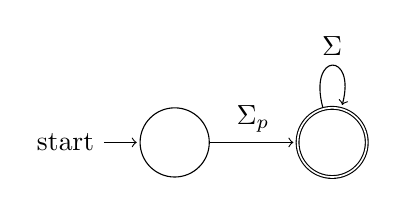
\begin{tikzpicture}[shorten >=1pt,node distance=2cm,on grid,auto] 
\node[state,initial] (q_1) {};
\node[state,accepting] (q_2) [right=of q_1] {};
\path[->]

(q_1) edge node {$\Sigma_p$} (q_2)
(q_2)
edge [loop above] node {$\Sigma$} ()
;
\end{tikzpicture}

Produce Buchi Automaton for \lstinline|(p -> (p U q))|.

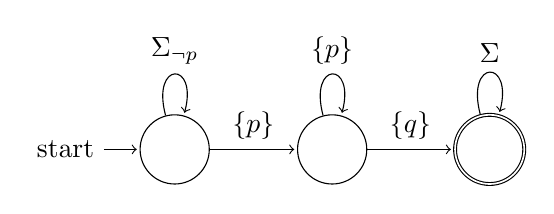
\begin{tikzpicture}[shorten >=1pt,node distance=2cm,on grid,auto] 
\node[state,initial] (q_1) {};
\node[state] (q_2) [right=of q_1] {};
\node[state,accepting] (q_3) [right=of q_2] {};
\path[->]

(q_1) edge node {$\{p\}$} (q_2)
edge [loop above] node {$\Sigma_{\lnot p}$} ()
(q_2) edge node {$\{q\}$} (q_3)
edge [loop above] node {$\{p\}$} ()
(q_3)
edge [loop above] node {$\Sigma$} ()
;
\end{tikzpicture}

\section*{Problem 2 Intersection Automaton}

Produce Buchi Automaton for $(a + b)^* b^\omega$ and $ab(a + b)^\omega$.

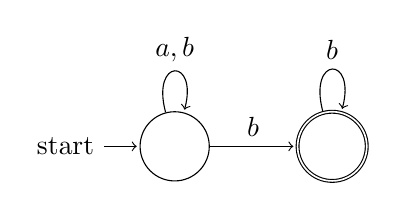
\begin{tikzpicture}[shorten >=1pt,node distance=2cm,on grid,auto] 
\node[state,initial] (q_1) {};
\node[state,accepting] (q_2) [right=of q_1] {};
\path[->]

(q_1) edge node {$b$} (q_2)
edge [loop above] node {$a, b$} ()
(q_2)
edge [loop above] node {$b$} ()
;
\end{tikzpicture}

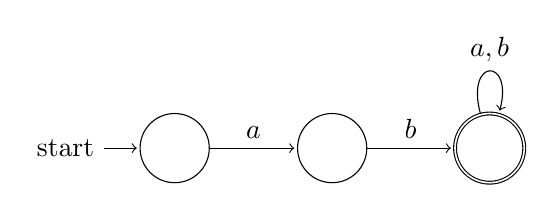
\begin{tikzpicture}[shorten >=1pt,node distance=2cm,on grid,auto] 
\node[state,initial] (q_1) {};
\node[state] (q_2) [right=of q_1] {};
\node[state,accepting] (q_3) [right=of q_2] {};
\path[->]

(q_1) edge node {$a$} (q_2)
(q_2) edge node {$b$} (q_3)
(q_3)
edge [loop above] node {$a, b$} ()
;
\end{tikzpicture}

And their intersection is $ab(a+b)^*b^\omega$.

\section*{Problem 3 Rendez-Vous Revisited}

Express the property with LTL
\begin{lstlisting}[frame=single]
ltl { <> (value == 100) }
\end{lstlisting}

and the verification failed as expected:
\begin{lstlisting}[frame=single]
% spin -a $<
% gcc -DMEMLIM=1024 -O2 -DXUSAFE -w -o pan pan.c
% ./pan -m10000 -a

pan:1: acceptance cycle (at depth 26)
pan: wrote p3.pml.trail
\end{lstlisting}

See file `p3.pml` for details.

\section*{Problem 4 Office Printer}

Add label `cs` to process `P` and process `Q`:
\begin{lstlisting}[frame=single]
if
:: usable ? true ->
cs:
printf("P printing...\n");
\end{lstlisting}

And verify with LTL:
\begin{lstlisting}[frame=single]
ltl not_starve { [] (<> (P@cs) \&\& <> (Q@cs)) }
\end{lstlisting}

Verify with SPIN:
\begin{lstlisting}[frame=single]
% spin -a $<
% gcc -DMEMLIM=1024 -O2 -DXUSAFE -w -o pan pan.c
% ./pan -m10000 -a
\end{lstlisting}

\section*{Problem 5 Verification with spin}

a) Failed verification
\begin{lstlisting}[frame=single]
ltl a { [] (count > 30) }
\end{lstlisting}
with or without weak-fairness.

b) Verify with LTL below
\begin{lstlisting}[frame=single]
ltl b { [] (
	(count > 0) -> ((count > 0) U (mode > 1))
	) }
\end{lstlisting}
No errors found if run with weak-fairness, but failed without weak-fairness. Without ensuring weak-fairness, process `n` might be never executed, and `mode > 1` never come true.

c) Below LTL
\begin{lstlisting}[frame=single]
ltl c { [] (
	(count > 0) -> (<> (count == 0))
	) }
\end{lstlisting}
always fail, with or without weak-fairness. Such routine exists:
\begin{lstlisting}[frame=single]
proc  1 (n:1) p5.pml:24 (state 1)	[mode = 3]
proc  0 (m:1) p5.pml:10 (state 1)	[mode = 1]
proc  0 (m:1) p5.pml:14 (state 5)	[(((mode==1)&&(count<30)))]
proc  0 (m:1) p5.pml:14 (state 6)	[count = (count+1)]
proc  0 (m:1) p5.pml:14 (state 5)	[(((mode==1)&&(count<30)))]
proc  0 (m:1) p5.pml:14 (state 6)	[count = (count+1)]
proc  0 (m:1) p5.pml:14 (state 5)	[(((mode==1)&&(count<30)))]
proc  0 (m:1) p5.pml:14 (state 6)	[count = (count+1)]
...
proc  0 (m:1) p5.pml:17 (state 12)	[else]
proc  1 (n:1) p5.pml:24 (state 1)	[mode = 3]
proc  0 (m:1) p5.pml:10 (state 1)	[mode = 1]
<<<<<START OF CYCLE>>>>>
proc  0 (m:1) p5.pml:17 (state 12)	[else]
proc  1 (n:1) p5.pml:24 (state 1)	[mode = 3]
proc  0 (m:1) p5.pml:10 (state 1)	[mode = 1]
\end{lstlisting}
That's why `count` will never be `0` again.

d) Without ensuring weak-fairness, following LTL
\begin{lstlisting}[frame=single]
ltl d { <> (mode == 3) } 
\end{lstlisting}
will fail, since process `n` can be never executed.

\section*{Problem 6 Never Claims}
The never claim ensure positive property `p` stay true. It's equivalent to such LTL
\begin{lstlisting}[frame=single]
ltl { [] (!p) }
\end{lstlisting}
`p6-1.pml' provided a model I win, and `p6-2.pml' provided a model the never claim win.

\end{document}